\section{Problemas Rutinarios}

\begin{itemize}
    \item Determine la ecuación de la recta tangente a la función \( f(x) = x^2 + 3x - 5 \) en \( x = 1 \).
\end{itemize}

\[m = \frac{y_2 - y_1}{x_2 - x_1}\]

\[m(x - x_1) = y - y_1\]

\[y = m(x - x_1) + y_1\]

\[f'(x) = 2x + 3\]

\[f'(1) = 5 = m\]

\[x_1 = 1\]

\[y_1 = f(x_1) = f(1) = 4\]

\textbf{Ecuación de la recta:}

\[y = 5(x - 1) + 4\]

\[f'(x) = 3x^2 - 12x + 9\]

\begin{itemize}
    \item Encuentre los puntos críticos y clasifíquelos como máximos, mínimos o puntos de silla para la función \(f(x)=x^3-6x^2+9x+2\)
\end{itemize}
\textbf{Los puntos criticos son aquellos donde la derivada vale cero}

\[
fx^2 - 12x + 9 = 0f\]

\[fx^2 - 4x + 3 = 0f\]

\[f(x - 3)(x - 1) = 0f\]

\[fx = 3 \quad \text{ó} \quad x = 1f\]

\[ff(3) = 2 \quad \quad f(1) = 6f\]

\begin{center}
    \begin{tabular}{|c|c|c|c|}
        \hline
        \textbf{Intervalos} & $(-\infty, 1)$ & $(1, 3)$ & $(3, \infty)$ \\
        \hline
        \textbf{Valor de Prueba} & $x = 0$ & $x = 2$ & $x = 4$ \\
        \hline
        \textbf{$f'(x)$} & $+$ & $-$ & $+$ \\
        \hline
        \textbf{Conclusión} & Crece & Decrece & Crece \\
        \hline
    \end{tabular}
\end{center}

\begin{itemize}
    \item $P(3, 2)$ es un máximo de la función.
    \item $P(1, 6)$ es un mínimo de la función.
\end{itemize}

\section*{Análisis de la continuidad de la función}

Sea la función:

\[
f(x) =
\begin{cases} 
x^2 - 1, & x < 2 \\
3x - 5, & x \geq 2
\end{cases}
\]

\subsection*{Condiciones de continuidad}

\begin{enumerate}
\item $f(a)$ existe:

\[f(2) = 3(2) - 5 = 1 \quad \checkmark\]

\item Verificamos si el límite lateral izquierdo y derecho son iguales:

\[\lim_{x \to a^-} f(x) = \lim_{x \to a^+} f(x)\]

Calculamos los límites laterales en $x = 2$:

\[\lim_{x \to 2^-} (x^2 -1) = 3\]

\[\lim_{x \to 2^+} (3x -5) = 1\]

Dado que:

\[3 \neq 1\]

Se concluye que el límite de $f(x)$ no existe, por lo tanto, \textbf{la función no es continua en $x=2$}. 
\end{enumerate}

\section*{Análisis de funciones}

\subsection*{\[f(x) = \frac{x}{x^2 - 1}\]}

\subsubsection*{Puntos de corte}

El punto de corte con el eje $y$:

\[f(0) = \frac{0}{0^2 - 1} = \frac{0}{-1} = 0\]

Por lo tanto, el punto de corte con el eje $y$ es:

\[y = 0, \quad x = 0\]

\subsubsection*{Dominio}

El denominador no debe ser igual a cero:

\[x^2 - 1 \neq 0\]

\[x \neq \pm 1\]

\subsubsection*{Asíntotas Verticales}

\[
\begin{array}{c|c|c}
x & -1.0 & -1.001 \\
\hline
\lim_{x \to 1^-} \frac{x}{(x+1)(x-1)} & -\infty & -\infty \\
\end{array}
\]

\[
\begin{array}{c|c|c}
x & -0.999 & 0.999 \\
\hline
\lim_{x \to 1^+} \frac{x}{(x+1)(x-1)} & \infty & \infty \\
\end{array}
\]

\[
\begin{array}{c|c|c}
x & -10 & -1001 \\
\hline
\lim_{x \to -1^-} \frac{x}{(x+1)(x-1)} & -\infty & -\infty \\
\end{array}
\]

\[
\begin{array}{c|c|c}
x & 0.99 & 0.999 \\
\hline
\lim_{x \to -1^+} \frac{x}{(x+1)(x-1)} & -499.7 & -499.9 \\
\end{array}
\]

\[
\begin{array}{c|c|c}
x & 1.01 & 1.001 \\
\hline
\lim_{x \to 1^+} \frac{x}{(x+1)(x-1)} & 500.2 & \infty \\
\end{array}
\]



\subsubsection*{Asíntotas Horizontales}

Calculamos el límite cuando $x \to \pm \infty$:

\[
\lim_{x \to \pm \infty} \frac{x}{x^2 - 1} = 0
\]

Por lo tanto, existe una asíntota horizontal en:

\[y = 0\]


\subsubsection*{Criterio de la Primera Derivada}

La primera derivada de la función es:

\[f'(x) = \frac{x^2 - 1 - \left[x \cdot 2x\right]}{(x^2 - 1)^2}\]

Simplificamos:

\[f'(x) = \frac{-x^2 - 1}{(x^2 - 1)^2} = 0\]

Resolviendo la ecuación:

\[-x^2 - 1 = 0\]

\[x^2 = -1\]

\[x = \pm \sqrt{-1}\]

Dado que $\sqrt{-1}$ no pertenece a los números reales ($\mathbb{R}$), concluimos que:

\[X \text{ no es un punto crítico}; X \notin \mathbb{R}\]

Por otro lado, la condición de discontinuidad se da cuando:

\[
x^2 - 1 \neq 0
\]

\[
x \neq \pm 1
\]

Por lo tanto, $x = \pm 1$ son puntos de discontinuidad.

\begin{center}
    \begin{tabular}{|c|c|c|c|}
        \hline
        Intervalos & $(-\infty,-1)$ & $(-1,1)$ & $(1,\infty)$ \\
        \hline
        Valor de Prueba & $x=-2$ & $x=0$ & $x=2$ \\
        \hline
        $f'(x)$ & - & - & - \\
        \hline
        Conclusión & Decrece & Decrece & Decrece \\
        \hline
    \end{tabular}
\end{center}


\subsubsection*{Criterio de la Segunda Derivada}

La primera derivada de la función es:

\[
f'(x) = \frac{-x^2 -1}{(x^2 - 1)^2}
\]

Calculamos la segunda derivada:

\[
f''(x) = - \frac{2x (x^2 -1)^2 - \left[ (x+1) \cdot 2 (x^2 -1) 2x \right]}{(x^2 -1)^4}
\]

\[
f''(x) = - \frac{2x (x^2-1)^2 - 4x (x^4 -1)}{(x^2 -1)^4}
\]

\[
f''(x) = \frac{2x(x^4 + 2x -3)}{(x^2 - 1)^4}
\]

Factorizamos:

\[
x^4 + 2x^2 -3
\]

Sea \( z = x^2 \), entonces:

\[
z^2 + 2z -3 = (z+3)(z-1)
\]

Sustituyendo:

\[
(x^2+3)(x^2-1)
\]

Por lo tanto, la segunda derivada queda:

\[
f''(x) = \frac{2x (x^2+3)}{(x^2 -1)^3}
\]

\subsubsection*{Puntos de inflexión y cambio de concavidad}

Para encontrar los puntos de inflexión, igualamos la segunda derivada a cero:

\[
2x(x^2+3) = 0
\]

Resolviendo:

\[
x = 0 \quad \Rightarrow \quad \text{Punto de inflexión}
\]

\[
x = \pm \sqrt{3} \quad \Rightarrow \quad \text{No es punto de inflexión}
\]

Ahora, analizamos los puntos donde el denominador de la segunda derivada se anula:

\[
(x^2 -1)^3 \neq 0
\]

\[
x^2 = 1 \quad \Rightarrow \quad x = \pm 1
\]

Estos corresponden a \textbf{puntos de cambio de concavidad}.

\begin{center}
    \begin{tabular}{|c|c|c|c|c|}
        \hline
        Intervalos & $(-\infty,-1)$ & $(-1,0)$ & $(0,1)$ & $(1,\infty)$ \\
        \hline
        Valor de Prueba & $x=-2$ & $x=-0.5$ & $x=0.5$ & $x=2$ \\
        \hline
        $f''(x)$ & - & + & - & + \\
        \hline
        Conclusión & Cóncava abajo ($\cap$) & Cóncava arriba ($\cup$) & Cóncava abajo ($\cap$) & Cóncava  arriba ($\cup$) \\
        \hline
    \end{tabular}
\end{center}

%%Segunda función
\subsection*{\[f(x) = \frac{1}{(x-1)(x-3)}\]}

\subsubsection*{Puntos de Corte:}

\[
f(0) = \frac{1}{3}
\]

\[
y = 0.33
\]

\[
X = \text{No Existe} \quad (1 \neq 0)
\]

\subsubsection*{Dominio:}

\[
(x-1) \neq 0 \quad \vee \quad (x-3) \neq 0
\]

\[
D_f = \mathbb{R} - \{1,3\}
\]

\subsubsection*{Asíntotas Verticales:}

\[
\begin{array}{c|c|c|c}
x & 0.9 & 0.99 & \cdots \\
\hline
\lim_{x \to 1^-} & 5 & 50 & \infty \\
\end{array}
\]

\[
\begin{array}{c|c|c|c}
x & 1.01 & 1.001 & \cdots \\
\hline
\lim_{x \to 1^+} & -50 & -500 & -\infty \\
\end{array}
\]

\[
\begin{array}{c|c|c|c}
x & 2.9 & 2.99 & \cdots \\
\hline
\lim_{x \to 3^-} & -5 & -50 & -\infty \\
\end{array}
\]

\[
\begin{array}{c|c|c|c}
x & 3.01 & 3.001 & \cdots \\
\hline
\lim_{x \to 3^+} & 50 & 500 & \infty \\
\end{array}
\]



\subsubsection*{Asíntotas Horizontales:}

\[
\lim_{x \to \pm\infty} \frac{1}{(x-1)(x-3)} = 0
\]

\[
\therefore \text{ Hay una asíntota en } y = 0
\]

\subsubsection*{Criterio de la Primera Derivada:}  

\[
f(x) = [(x - 1)(x - 3)]^{-1}
\]

La derivada de \( f(x) \) es:
\[
f'(x) = -[(x - 1)(x - 3)]^{-2} \cdot [(x - 3) + (x - 1)]
\]

Simplificando:
\[
f'(x) = \frac{-2x + 4}{[(x - 1)(x - 3)]^2}
\]

Resolviendo \( -2x + 4 = 0 \):  
\[
x = 2 \implies f(2) = -1 \quad \textbf{Punto Crítico}
\]

Restricciones del dominio:
\[
(x - 1) \neq 0 \implies x \neq 1 \quad \textbf{Pto. de Discontinuidad}
\]
\[
(x - 3) \neq 0 \implies x \neq 3 \quad \textbf{Pto. de Discontinuidad}
\]

%%Quinta tabla

\begin{center}
    \begin{tabular}{|c|c|c|c|c|}
        \hline
        Intervalos & $(-\infty,1)$ & $(1,2)$ & $(2,3)$ & $(3,\infty)$ \\
        \hline
        Valor de Prueba & $x=0$ & $x=1.5$ & $x=2.5$ & $x=4$ \\
        \hline
        $f'(x)$ & $+$ & $+$ & $-$ & $-$ \\
        \hline
        Conclusión & Crece & Crece & Decrece & Decrece \\
        \hline
    \end{tabular}
\end{center}


\subsubsection*{Criterio de la 2da Derivada:}

\[
f'(x) = \frac{-2x + 4}{[ (x - 1)(x - 3) ]^2}
\]

\[
f'(x) = \frac{-2x + 4}{(x^2 - 4x + 3)^2}
\]

\[
f''(x) = \frac{-2 (x^2 - 4x + 3)^2 - [ (-2x + 4) \cdot 2 (x^2 - 4x + 3) (2x - 4) ]}{(x^2 - 4x + 3)^4}
\]

\[
f''(x) = \frac{-2 (x^2 - 4x + 3)^2 - (-2x + 4) (x^2 - 4x + 3) (2x - 4)}{(x^2 - 4x + 3)^4}
\]

\[
f''(x) = \frac{(x^2 - 4x + 3) \left[ -2 (x^2 - 4x + 3) - (-4x + 8) (2x - 4) \right]}{(x^2 - 4x + 3)^4}
\]

\[
f''(x) = \frac{-2 (x^2 - 4x + 3) + (4x - 8) (2x - 4)}{(x^2 - 4x + 3)^3}
\]

\[
f''(x) = \frac{-2x^2 + 8x - 6 + 8x^2 - 16x - 16x + 32}{(x^2 - 4x + 3)^3}
\]

\[
f''(x) = \frac{6x^2 - 24x + 26}{(x^2 - 4x + 3)^3}
\]

\[
6x^2 - 24x + 26 = 0
\]

\[
3x^2 - 12x + 13 = 0
\]

\[
\sqrt{b^2 - 4ac}
\]

\[
\sqrt{144 - 156}
\]

\[
3x^2 - 12x + 13 = 0
\]
\[
x^2 - 4x + 3 = 0
\]

\[
(x - 3)(x - 1) = 0
\]

\subsubsection*{Pts. de Cambio de Concavidad}

\[
x = 3 \quad x = 1
\]

% Cuarta tabla (concavidad)
\begin{center}
    \begin{tabular}{|c|c|c|c|}
        \hline
        Intervalos & $(-\infty,1)$ & $(1,3)$ & $(3,\infty)$ \\
        \hline
        Valor de Prueba & $x=0$ & $x=2$ & $x=4$ \\
        \hline
        $f''(x)$ & + & - & + \\
        \hline
        Conclusión & Cóncava arriba ($\cup$) & Cóncava abajo ($\cap$) & Cóncava arriba ($\cup$) \\
        \hline
    \end{tabular}
\end{center}

\begin{figure}[H]
    \centering
    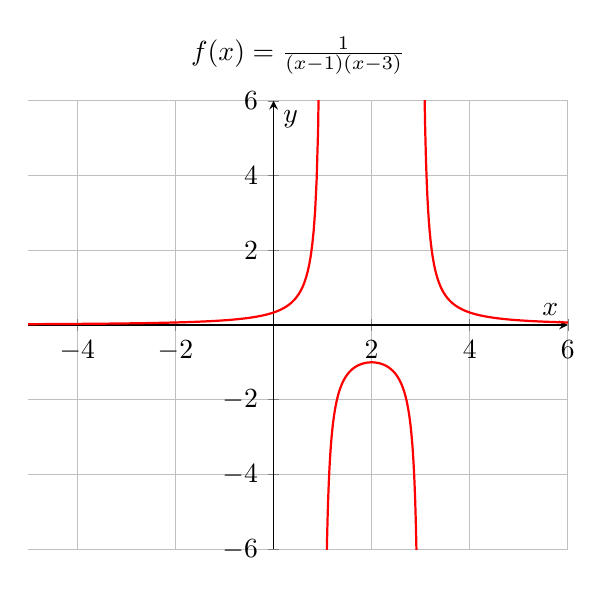
\begin{tikzpicture}
    \begin{axis}[
      title={$f(x) = \frac{1}{(x-1)(x-3)}$},
        axis lines = middle,
        grid = major,
        xmin = -5, xmax = 6,   % Ajusta la ventana en x
        ymin = -6, ymax = 6,   % Ajusta la ventana en y
        xlabel={$x$},
        ylabel={$y$},
        unbounded coords=jump, % Salta en lugar de trazar líneas infinitas
        samples=200            % Más puntos para una curva suave
    ]
    % Graficar f(x) en tres intervalos separados:
    %  1) Desde x=-5 hasta justo antes de x=1
    \addplot[domain=-5:0.999, thick, red]
      {1/((x-1)*(x-3))};

    %  2) Desde un poco después de x=1 hasta antes de x=3
    \addplot[domain=1.001:2.999, thick, red]
      {1/((x-1)*(x-3))};

    %  3) Desde un poco después de x=3 hasta x=6
    \addplot[domain=3.001:6, thick, red]
      {1/((x-1)*(x-3))};

    \end{axis}
\end{tikzpicture}
\end{figure}


\section*{\[f(x) = x + \frac{1}{x^2}\]}

\subsubsection*{Puntos de Corte:}

\[
f(x) = \frac{x^3 + 1}{x^2}
\]

\[
x^3 + 1 = 0
\]

\[
x = \sqrt[3]{-1}
\]

\[
x = -1
\]

\[
y \text{ no existe}
\]

\subsubsection*{Dominio:}

\[
x \neq 0 \quad D_f = \mathbb{R} - \{0\}
\]

\subsubsection*{Asíntotas Verticales:}

\[
\begin{array}{c|c|c|c}
x & -0.01 & -0.001 & \cdots \\
\hline
\lim_{x \to 0^-} & 9999.9 & 999999 & \infty
\end{array}
\]

\[
\begin{array}{c|c|c|c}
x & 0.01 & 0.001 & \cdots \\
\hline
\lim_{x \to 0^+} & 10^4 & 10^6 & \infty
\end{array}
\]


\subsubsection*{Asíntotas Horizontales:}

\[
\lim_{x \to \infty} \frac{x^3 - 1}{x^2} = \infty
\]

\[
\lim_{x \to -\infty} \frac{x^3 - 1}{x^2} = -\infty
\]

Hay 2 asíntotas oblicuas.

\subsubsection*{Criterio de la Primera Derivada:}

\[
f(x) = x + \frac{1}{x^2}
\]

\[
f'(x) = 1 + \left(-\frac{2}{x^3}\right)
\]

\[
f'(x) = 1 - \frac{2}{x^3}
\]

\[
\frac{2}{x^3} = 1 \implies x = \sqrt[3]{2}
\]

\[
x \approx 1.26 \quad f(\sqrt[3]{2}) \approx 1.89
\]

\textbf{Punto Crítico}: \(x \approx 1.26\)

\[
x^2 \neq 0 \implies x \neq 0
\]

\textbf{Punto de Discontinuidad}: \(x = 0\)

% Penultima tabla (crecimiento y decrecimiento)
\begin{center}
    \begin{tabular}{|c|c|c|c|}
        \hline
        Intervalos & $(-\infty,0)$ & $(0,\sqrt[3]{2})$ & $(\sqrt[3]{2},\infty)$ \\
        \hline
        Valor de Prueba & $x=-1$ & $x=1$ & $x=2$ \\
        \hline
        $f'(x)$ & + & - & + \\
        \hline
        Conclusión & Crece & Decrece & Crece \\
        \hline
    \end{tabular}
\end{center}

\subsubsection*{Criterio de la Segunda Derivada:}

\[
f'(x) = 1 - 2x^{-3}
\]

\[
f''(x) = 6x^{-4}
\]

\[
f''(x) = \frac{6}{x^4}
\]

\[
0 \neq 6
\]

\textbf{No hay puntos de inflexión}

\[
x^4 \neq 0 \implies x \neq 0
\]

\textbf{Punto de Cambio de Concavidad}: \(x \neq 0\)

% Ultima tabla (concavidad)
\begin{center}
    \begin{tabular}{|c|c|c|}
        \hline
        Intervalos & $(-\infty,0)$ & $(0,\infty)$ \\
        \hline
        Valor de Prueba & $x=-1$ & $x=1$ \\
        \hline
        $f''(x)$ & + & + \\
        \hline
        Conclusión & Cóncava hacia arriba ($\cup$) & Cóncava hacia arriba ($\cup$) \\
        \hline
    \end{tabular}
\end{center}


\begin{figure}[H]
    \centering
    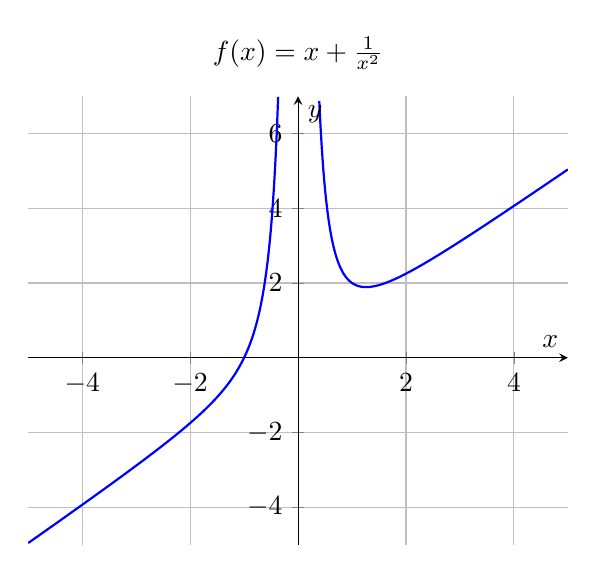
\begin{tikzpicture}
    \begin{axis}[
        title={$f(x) = x + \frac{1}{x^2}$},
        axis lines = middle,
        grid = major,
        xlabel={$x$},
        ylabel={$y$},
        xmin=-5, xmax=5,      % Ajusta la ventana en x
        ymin=-5, ymax=7,      % Ajusta la ventana en y
        restrict y to domain=-5:7, % Corta valores de y fuera de [-5,7]
        unbounded coords=jump, % Salta las discontinuidades en vez de trazar líneas infinitas
        samples=200
    ]
    % Dividimos el dominio en 2 intervalos para evitar x=0 (asíntota vertical)
    \addplot[domain=-5:-0.2, thick, blue] {x + 1/(x^2)};
    \addplot[domain=0.2:5, thick, blue] {x + 1/(x^2)};
    \end{axis}
\end{tikzpicture}
\end{figure}



